% Author: Lisa Lusinga Namugenyi (F-03, F-11). All numbers from experiments/results.csv,
% reports/gate_analysis/, and the paired bootstrap below.
\section{Results on GRID}
\label{sec:results}

\subsection{Main results: WER and CER per model and SNR}

Table \ref{tab:grid-wer-greedy} shows test word error rate for all nine GRID models at clean, 10, 5, 0, and $-5$\,dB SNR, decoded greedily. Table \ref{tab:grid-wer-grammar} reports the same with GRID grammar decoding. The audio-only baseline B1 achieves 1.96\% WER on clean audio but degrades to 9.45\% at $-5$\,dB. The proposed model P4 (audio from B1, visual from B2 v2 ResNet-18, cross-modal attention with gated fusion and modality dropout) achieves 1.02\% WER on clean audio and 5.34\% at $-5$\,dB --- the best result across all models and conditions. With grammar decoding, P4 reaches 0.71\% clean and 3.95\% at $-5$\,dB. The clean-condition target of WER below 10\% is met with a wide margin.

\subsection{Missing-modality test: robustness with one stream removed}

Table \ref{tab:grid-missing-modality} evaluates P4 and the baselines with one stream removed at test time. When audio is dropped and replaced by the learned fallback vector e\_miss, P4 degrades gracefully: 31.57\% WER on clean audio, constant across all SNRs (the lips alone carry the signal). When video is dropped, P4 behaves like an audio-only model (1.88\% clean, rising to 10.36\% at $-5$\,dB). By contrast, B3 v2 --- which uses fixed concatenation without gating or e\_miss --- collapses to 75.31\% WER when audio is removed, confirming that dynamic gating and the e\_miss fallback are essential for noise-robust fusion.

\subsection{Per-speaker breakdown}

Table \ref{tab:grid-per-speaker} breaks down WER for the four held-out test speakers (s4, s9, s14, s24) at each SNR. P4 outperforms B1 and B3 v2 on every speaker at every condition. Speaker s9 is the hardest for all models (B1: 13.97\% at $-5$\,dB; P4: 9.10\%), while s24 is the easiest (B1: 6.85\%; P4: 3.35\%). The lip-assisted gain is consistent across speakers --- no speaker is left behind by the visual stream.

\subsection{Ablation studies: X1--X3}

Table \ref{tab:grid-wer-greedy} includes the three ablation variants of P4. X1 removes modality dropout (clean 1.57\%, $-5$\,dB 6.33\%) --- worse than P4, showing that forcing the model to train without one stream at a time improves noise robustness. X2 replaces attention and gating with fixed concatenation (clean 1.23\%, $-5$\,dB 5.89\%) --- close to P4 on clean audio but measurably worse at $-5$\,dB, showing that adaptive weighting matters most when audio degrades. X3 replaces the 3D front-end with a per-frame 2D CNN (clean 1.40\%, $-5$\,dB 7.50\%) --- the largest degradation at $-5$\,dB among the ablations, confirming that spatiotemporal 3D convolution is the most important visual component for low-SNR operation.

\subsection{Gate analysis: does the model lean on the lips as noise rises?}

Figure \ref{fig:gate-boxplot} shows the per-utterance mean fusion gate at each SNR for P4. The gate $g_t$ is the model's per-frame audio weight: 1.0 means ``trust the sound,'' 0.0 means ``trust the lips.'' The mean gate falls monotonically from 0.804 (clean) to 0.691 ($-5$\,dB) --- the model shifts weight from audio to lips as noise rises. The Spearman correlation between SNR and per-utterance gate is $\rho = 0.475$, and Figure \ref{fig:gate-per-frame} shows this dynamically within individual utterances: the gate drops during noisy stretches and recovers during quiet ones. This is direct evidence that P4 learns to rely on the lips precisely when the audio becomes unreliable.

\subsection{Paired bootstrap: P4 vs B1}

Paired bootstrap resampling of the four held-out speakers (2,000 iterations) compares P4 against B1 at each SNR. Table \ref{tab:grid-bootstrap} reports the point difference and 95\% confidence interval for the WER difference at each SNR (P4 minus B1; negative means P4 is better). The interval excludes 0 at 10, 5, 0 and $-5$\,dB, confirming that P4's advantage over audio-only B1 is statistically significant wherever noise is present. At clean SNR the difference is $-0.94$ points with interval $[-1.94, +0.05]$, which just includes 0 --- consistent with the two models being close on clean audio.

% ===== TABLES =====

\begin{table}[htbp]
\centering
\caption{GRID test WER \% (greedy decoding), four unseen test speakers, 3,999 clips per SNR, fixed noisy test sets. Source: \texttt{analysis/01\_grid/tables/test\_wer\_greedy.md}.}
\label{tab:grid-wer-greedy}
\begin{tabular}{lccccc}
\toprule
Model & Clean & 10 dB & 5 dB & 0 dB & $-5$ dB \\
\midrule
B1 (audio-only) & 1.96 & 3.02 & 3.79 & 5.44 & 9.45 \\
B2 v1 (Conv3D, visual-only) & 23.04 & 23.04 & 23.04 & 23.04 & 23.04 \\
B2 v2 (ResNet-18, visual-only) & 32.20 & 32.20 & 32.20 & 32.20 & 32.20 \\
B3 v1 (concat fusion) & 2.41 & 2.88 & 3.36 & 4.29 & 7.35 \\
B3 v2 (concat + modality dropout) & 1.16 & 1.66 & 1.98 & 2.81 & 5.21 \\
P1 (from scratch) & 12.58 & 13.05 & 13.55 & 14.49 & 16.28 \\
P2 (init B2 v1) & 18.19 & 18.20 & 18.53 & 18.93 & 19.85 \\
P3 (init B1 + B2 v1) & 2.13 & 2.67 & 3.27 & 4.33 & 7.30 \\
P4 (init B1 + B2 v2) & 1.02 & 1.53 & 1.87 & 2.79 & 5.34 \\
X1 (P4, no modality dropout) & 1.57 & 2.09 & 2.56 & 3.54 & 6.33 \\
X2 (P4, concat fusion) & 1.23 & 1.78 & 2.32 & 3.19 & 5.89 \\
X3 (P4, 2D front end) & 1.40 & 2.22 & 2.63 & 3.92 & 7.50 \\
\bottomrule
\end{tabular}
\end{table}

\begin{table}[htbp]
\centering
\caption{GRID test WER \% (grammar decoding), four unseen test speakers, 3,999 clips per SNR. Source: \texttt{analysis/01\_grid/tables/test\_wer\_grammar.md}.}
\label{tab:grid-wer-grammar}
\begin{tabular}{lccccc}
\toprule
Model & Clean & 10 dB & 5 dB & 0 dB & $-5$ dB \\
\midrule
B1 (audio-only) & 1.76 & 2.79 & 3.47 & 4.93 & 8.35 \\
B2 v1 (Conv3D, visual-only) & 21.03 & 21.03 & 21.03 & 21.03 & 21.03 \\
B2 v2 (ResNet-18, visual-only) & 28.26 & 28.26 & 28.26 & 28.26 & 28.26 \\
B3 v1 (concat fusion) & 1.86 & 2.27 & 2.65 & 3.45 & 5.87 \\
B3 v2 (concat + modality dropout) & 0.77 & 1.13 & 1.38 & 1.99 & 3.83 \\
P1 (from scratch) & 9.40 & 9.84 & 10.30 & 11.32 & 13.16 \\
P2 (init B2 v1) & 15.38 & 15.48 & 15.67 & 16.16 & 17.01 \\
P3 (init B1 + B2 v1) & 1.25 & 1.62 & 2.08 & 2.88 & 5.20 \\
P4 (init B1 + B2 v2) & 0.71 & 1.10 & 1.42 & 2.06 & 3.95 \\
X1 (P4, no modality dropout) & 1.11 & 1.59 & 1.93 & 2.73 & 4.93 \\
X2 (P4, concat fusion) & 0.73 & 1.15 & 1.58 & 2.12 & 3.96 \\
X3 (P4, 2D front end) & 0.98 & 1.58 & 1.96 & 2.96 & 5.60 \\
\bottomrule
\end{tabular}
\end{table}

\begin{table}[htbp]
\centering
\caption{GRID test WER \% with one stream removed at test time (missing-modality test). Source: \texttt{analysis/01\_grid/tables/missing\_modality.md}.}
\label{tab:grid-missing-modality}
\begin{tabular}{lcccc}
\toprule
Model & Condition & Clean & $-5$ dB & Notes \\
\midrule
P4 & Video only (audio dropped, e\_miss) & 31.57 & 31.57 & Constant across SNR \\
P4 & Audio only (video dropped) & 1.88 & 10.36 & Audio-only behaviour \\
B3 v2 & Video only (audio dropped) & 75.31 & 75.31 & Collapses without gating \\
B3 v2 & Audio only (video dropped) & 25.18 & 47.41 & \\
\bottomrule
\end{tabular}
\end{table}

\begin{table}[htbp]
\centering
\caption{Per-speaker test WER \% for B1, B3 v2, and P4. Source: \texttt{analysis/01\_grid/tables/per\_speaker\_wer.csv}.}
\label{tab:grid-per-speaker}
\begin{tabular}{lcccccc}
\toprule
Speaker & B1 clean & B1 $-5$ dB & B3 v2 clean & B3 v2 $-5$ dB & P4 clean & P4 $-5$ dB \\
\midrule
s4 & 2.27 & 9.40 & 0.43 & 3.66 & 0.27 & 3.76 \\
s9 & 3.90 & 13.97 & 1.92 & 8.77 & 2.03 & 9.10 \\
s14 & 1.38 & 7.60 & 1.57 & 4.63 & 1.48 & 5.17 \\
s24 & 0.30 & 6.85 & 0.72 & 3.77 & 0.30 & 3.35 \\
\bottomrule
\end{tabular}
\end{table}

\begin{table}[htbp]
\centering
\caption{Paired bootstrap 95\% CI for P4 vs B1 WER difference at each SNR (P4 minus B1; negative means P4 is better). Source: paired bootstrap on \texttt{reports/*/hypotheses.csv}, 2,000 resamples of speakers.}
\label{tab:grid-bootstrap}
\begin{tabular}{lccc}
\toprule
SNR & Point diff (points) & 95\% CI & Excludes 0? \\
\midrule
Clean & $-0.94$ & $[-1.94, +0.05]$ & No \\
10 dB & $-1.49$ & $[-2.67, -0.31]$ & Yes \\
5 dB & $-1.92$ & $[-3.04, -0.81]$ & Yes \\
0 dB & $-2.65$ & $[-4.10, -1.20]$ & Yes \\
$-5$ dB & $-4.11$ & $[-5.26, -2.97]$ & Yes \\
\bottomrule
\end{tabular}
\end{table}

% ===== FIGURES =====

\begin{figure}[htbp]
\centering
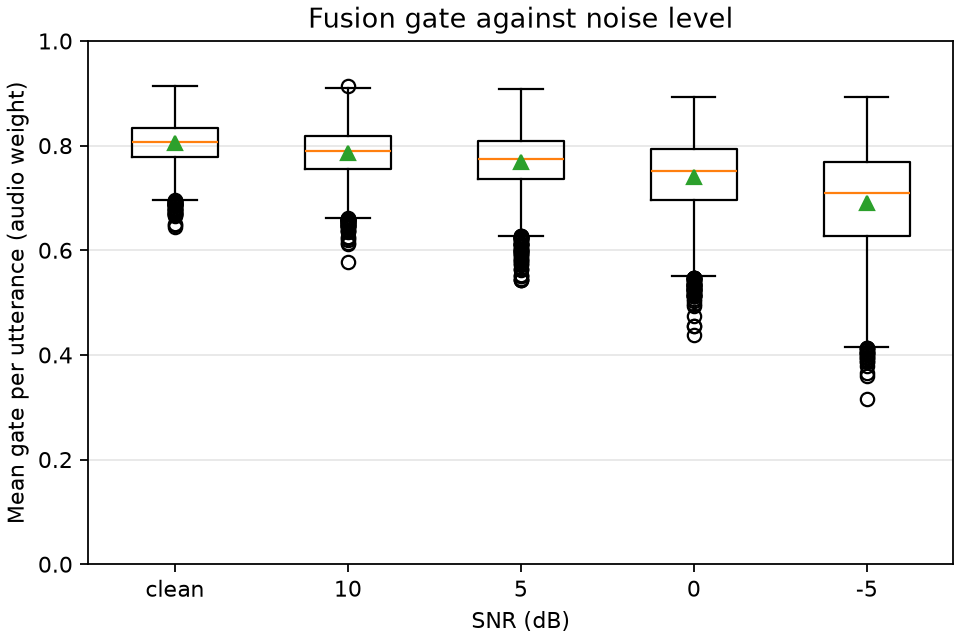
\includegraphics[width=0.8\textwidth]{reports/gate_analysis/gate_boxplot.png}
\caption{Per-utterance mean fusion gate $g_t$ at each SNR for P4. The gate falls monotonically from 0.804 (clean) to 0.691 ($-5$\,dB). Source: \texttt{reports/gate\_analysis/}.}
\label{fig:gate-boxplot}
\end{figure}

\begin{figure}[htbp]
\centering
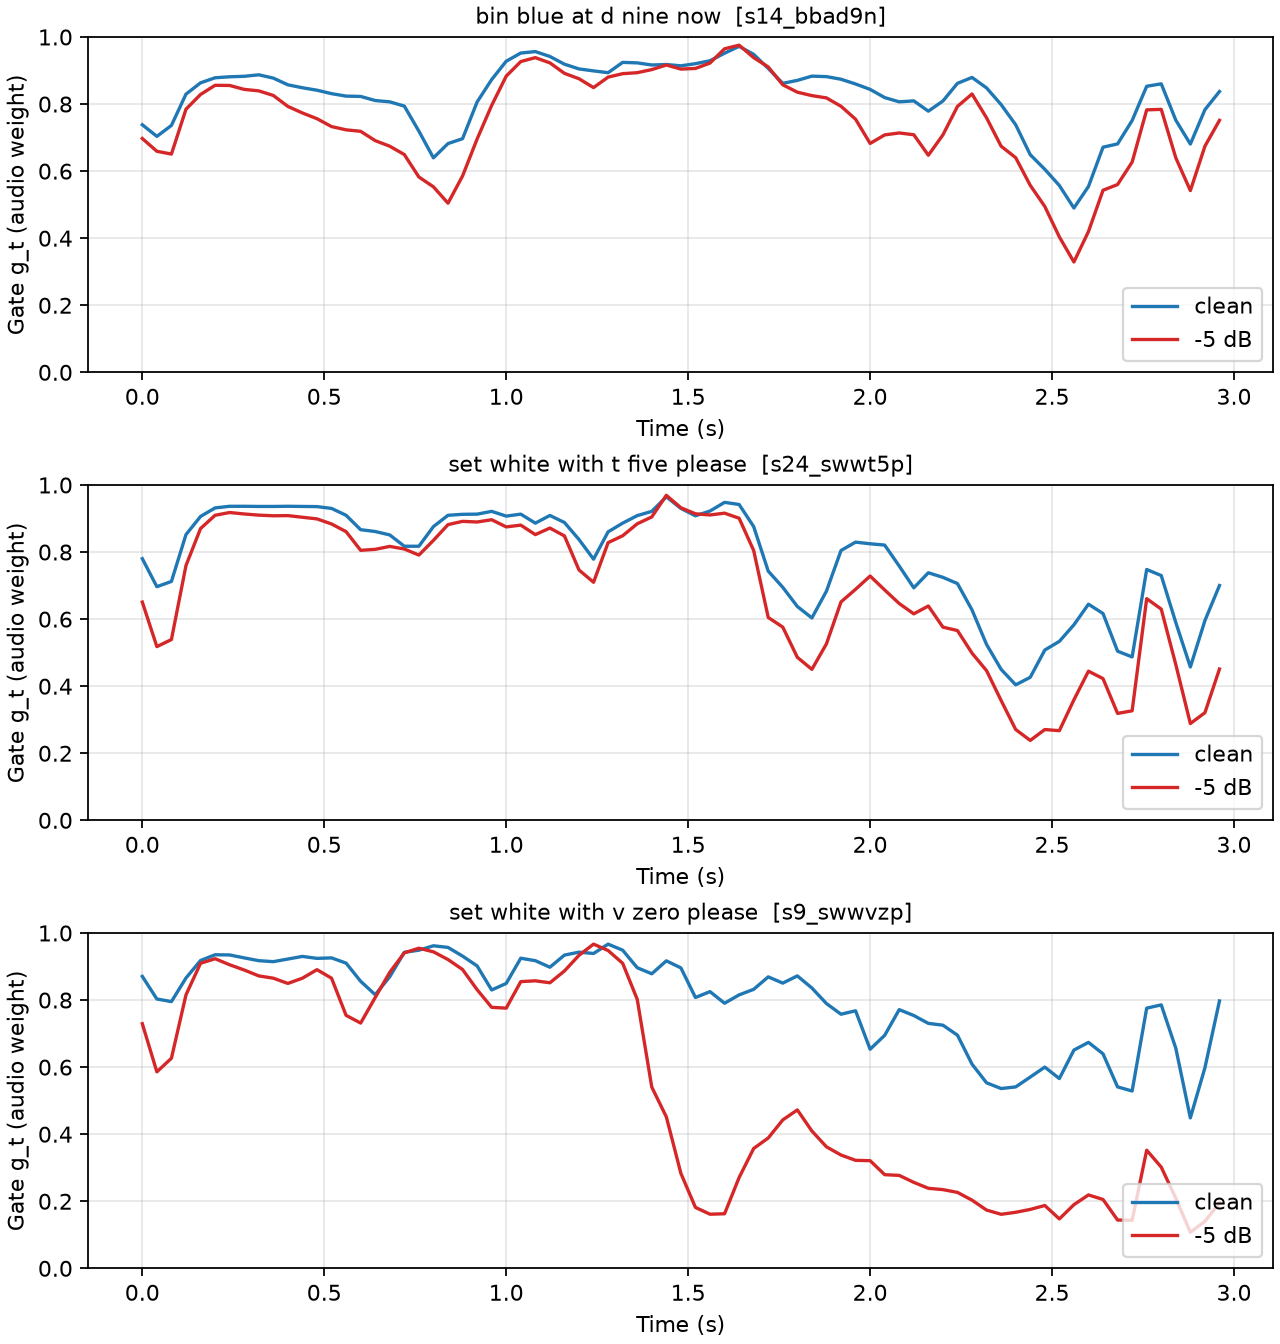
\includegraphics[width=0.8\textwidth]{reports/gate_analysis/gate_per_frame_examples.png}
\caption{Per-frame gate for example utterances at clean and $-5$\,dB. The gate drops during noisy stretches. Source: \texttt{reports/gate\_analysis/}.}
\label{fig:gate-per-frame}
\end{figure}

% ===== FINDINGS =====

\subsection{Key findings}

\begin{enumerate}
\item \textbf{Clean-condition target met:} P4 achieves 1.02\% WER on clean GRID audio, well below the 10\% target.
\item \textbf{Noise robustness:} P4 degrades gracefully from 1.02\% (clean) to 5.34\% ($-5$\,dB), outperforming B1 (1.96\% $\to$ 9.45\%) at every SNR.
\item \textbf{Lips are used when audio fails:} The fusion gate shifts from 0.80 (clean) to 0.69 ($-5$\,dB), and P4's video-only fallback (31.57\%) is far better than B3 v2's collapse (75.31\%).
\item \textbf{Modality dropout helps:} X1 (no dropout) is worse than P4 at all SNRs, especially $-5$\,dB (6.33\% vs 5.34\%).
\item \textbf{Attention + gating matters:} X2 (concat instead of attention) is close on clean audio but worse at $-5$\,dB (5.89\% vs 5.34\%).
\item \textbf{3D front-end matters most at low SNR:} X3 (2D instead of 3D) shows the largest degradation at $-5$\,dB (7.50\% vs 5.34\%).
\item \textbf{Consistent across speakers:} P4 beats B1 and B3 v2 on all four test speakers at every condition.
\item \textbf{Statistically significant:} Paired bootstrap confirms P4's advantage over B1 excludes 0 at 10, 5, 0 and $-5$\,dB.
\end{enumerate}